\chapter{Theoretical Overview}
\label{ch:theory}
 
The field of particle physics endeavours to build a full description of the dynamics of the fundamental particles and interactions which govern the universe. Progress is made through both theoretical postulation and experimental finding. The theoretical branch seeks to describe mathematically the framework that reflect the symmetries in nature, through the construction of models. These are constructed to describe observed behaviour and to predict that not yet observed. The description of current understanding is collectively known as the Standard Model (SM), and is a rigorously tested and widely accepted theory. However, whilst there are no disagreements, there are some gaps which hint at physics beyond, fuelling many new theories that predict new physics beyond. This leads in turn to a  new generation of experimentalists seeking answers to what lies at the next energy frontier.

\section{The Standard Model}

The Standard Model (SM) is the name given to the theories that successfully describe the known elementary particles and their fundamental interactions with respect to the strong, weak and electromagnetic forces. There are two main types of fundamental particle, which in order to distinguish requires the introduction of the concept of spin.

\begin{description}
\item[Spin] \hfill \\
Spin is the name given to a property of elementary particles, corresponding to a type of angular momentum, although this differs from classical angular momentum. This is an intrinsic property and thus has a specific value for each particle type. It can be thought of for composite particles as the angular momentum about the central point, but it is known that elementary particles carry spin also, despite being point particles with no internal structure, so this analogy breaks down. The values of the spin quantum number $s$ which describe the magnitude can take any half integer value $s=0, \frac{1}{2}, 1, \frac{3}{2}$, etc. In addition to magnitude we describe a particle as having spin \textit{up} (positive) when the spin is in the direction of the z-axis, and spin \textit{down} (negative) if the spin is against the direction of the z-axis. 

The definition of spin gives rise to a second key property, known as chirality. When the spin direction is in the direction of momentum of the particle it is described as left-handed, and when it is against as right-handed. The chirality of a particle is integral to the way it behaves, as will be seen in the treatment of the weak force. In the massless limit  the chirality is analogous to another concept, that of helicity, although it is worth noting that for a massive particle helicity depends on the reference frame of observation, wheres chirality describes an inherent property that determines how the particle will behave.
\end{description}
All fundamental particles are divided into the spin-1/2 \textit{fermions} which are the building blocks for matter, and the force-mediating \textit{bosons} which must carry integer spin, usually spin-1.  A particle's spin dictates how it behaves, as the wave function of a bosonic system is symmetric under the swap of two of its particles, whilst that of a fermionic system is anti-symmetric. A consequence of this, as can be seen in Equation \ref{eqn:pauli} is the well-known Pauli Exclusion Principle, that two fermions may not exist in the same state. 

\begin{equation}
\psi_{f}(x_{a},x_{b}) = -\psi_{f}(x_{b},x_{a}), \quad \therefore \quad \psi_{f}(x_{a},x_{a}) = 0
\label{eqn:pauli}
\end{equation}
 
 
Each fermion can be described as a spinor field $\psi$ which describes a pair of complex fields, the left-handed ($\psi_{L}$) and right-handed ($\psi_{R}$) representations. All visible matter is made out of fermions, which can be described in three families, or ``generations", each of which is further divided into two sets, the quarks and the leptons. There are three charged leptons with one unit (negative) of electric charge, e, the electron (e$^{-}$), the muon ($\mu^{-}$) and the tau ($\tau^{-}$), and three associated massless or incredibly light  neutral leptons called neutrinos that are named after the charged lepton in their generation, $\nu_{e}$, $\nu_{\mu}$ and $ \nu_{\tau}$ respectively. This indicates the introduction of a new concept, ``flavour", of which there are three, one for each generation. 

The quarks show an analogous structure, divided into two types dependent on electric charge carried, each with three generations. The up (u), charm (c) and top (t) quarks carry $+\sfrac{2}{3}$ e while the down (d), strange (s) and bottom (b) quarks carry $-\sfrac{1}{3}$ e. Each of the 6 quarks corresponds to its own flavour. 

The generation structure is shown in Equation~\ref{eqn:threefams}. The particles in the second and third generation exhibit the same properties as the corresponding first generation particles, except for the mass which increases with ascending generations. The first generation is therefore stable and all ordinary matter is constructed from it, whilst the second and third, once produced, decay into particles of the first generation. In addition to each particle detailed here, there exists a corresponding antiparticle due to a symmetry in charge and quantum numbers.
 
\begin{equation}
\begin{bmatrix}
\nu_{e} & u \\
e & d \\
\end{bmatrix},
\begin{bmatrix}
\nu_{\mu} & c \\
\mu & s \\
\end{bmatrix},
\begin{bmatrix}
\nu_{\tau} & t \\
\tau & b\\
\end{bmatrix}
\label{eqn:threefams}
\end{equation}

The bosons are force mediating particles, the photon $\gamma$ for the electromagnetic force, the 8 gluons $g_{i}$ for the strong force and the $W^{\pm}$ and Z bosons that carry the weak (nuclear) force, all of which are spin-1 particles. The photon and gluons are massless, whilst the weak vector bosons have non-negligible mass. The final particle of the SM is the Higgs Boson of spin-0, as yet undiscovered in experiment but expected from the theory, as will be detailed later. 

\subsection{Gauge Theory of Interactions}

The theories that make up the SM are formulated mathematically using Quantum Field Theory (QFT), in which particles are thought of as excitations of fields, and the dynamics of a given system are summarised in what is known as Lagrangian formalism. In this formalism the Lagrangian L is the difference between kinetic energy T and potential energy V, $L = T - V$. In QFT it is usual to describe a system by the Lagrangian Field Density $\Lagr$, where L is obtained from $\Lagr$ by integrating over the spatial component $d^{3}x$.


In order to reflect the symmetries observed in nature, the dynamics of a system and therefore the Lagrangian Density $\Lagr$, must be invariant under some set of transformations. For example, a generic phase $\alpha$ may be added,

\begin{equation}
\psi \rightarrow e^{-i\alpha}\psi, 
\label{GlobalTrans}
\end{equation}


where $\psi$ represents a spinor field. If $\alpha$ has no reliance on the space-time coordinate, we say this is a global symmetry. In order to describe the fundamental interactions it is necessary to use the special case where the transformations are \textit{local}, where $\alpha$ has a dependence on the space-time coordinate. The Standard Model describes such symmetries, a case we call gauge invariance, and is a special case of field theory known as Gauge Theory, where the transformations have the form, 


\begin{equation}
\psi(\stc) \rightarrow e^{-i\alpha(\stc)}\psi (\stc).
\label{LocalTrans}
\end{equation}


It is clear that $\Lagr$ will not remain unchanged by such a transformation, as the dependence of $\alpha$ on $x$ means that the coordinate derivative $\partial_{\mu}$ introduces extra terms. In order to leave the Lagrangian unchanged a vector field is introduced $A_{\mu}$ that transforms under another local transformation to keep $\Lagr$ constant: 

\begin{equation}
A_{\mu} \rightarrow A_{\mu} + \frac{1}{g} \partial_{\mu} \alpha(\stc).
\label{ATrans}
\end{equation}

Thus we can rewrite $\Lagr$ introducing the \textit{covariant derivative}, 
\begin{equation}
\slashed{\Dev}_{\mu} = \partial_{\mu} - igA_{\mu}. 
\end{equation}

This interaction between the spinor field and the vector field through this covariant derivative indicate the interactions of matter particles though the force carrying bosons. From Noether's Theorem, it is known that as a consequence of a symmetry in a dynamical system there is an associated physically conserved quantity~\cite{Rolnick}. Just as the classical conservation laws pertaining to momentum and energy are given by the space-time translational symmetries in Classical Mechanics, for the electromagnetic force symmetries in Quantum Mechanics the electric charge is conserved. Analogously, there ought to be conserved ``charges" for the strong and weak forces also, corresponding to quantum numbers from their Lagrangian Densities. 
 
The set of possible transformations is described in the language of Group Theory, and thus we describe the SM as a non-Abelian Yang-Mills type gauge field theory based on the symmetry group $SU(3)_{C} \times SU(2)_{L} \times U(1)_{Y}$. As this group is a product, the three individual elements are free to each have their own coupling constant, and these may differ. The strong interactions described by Quantum Chromodynamics (QCD) are represented by $SU(3)_{C}$, labelled C to indicate the conserved charge ``Colour". The electromagnetic and weak interactions are represented together due to Electroweak Unification, which we shall explore in detail later, by the group $SU(2)_L \times U(1)_{Y}$ where L stands for left, indicating the parity violation of the weak interaction and Y the conserved charge ``hypercharge". As of yet, the fourth fundamental force Gravity is not included in the Standard Model, but this is seen as of little consequence to particle physics as gravitational forces have comparatively little effect on fundamental particles at current experimental energy scales. 

\subsubsection{Quantum Electrodynamics}

The fundamental electromagnetic force is studied in quantum field theory as Quantum ElectroDynamics (QED), the oldest and simplest of the theories brought together to form the SM. The symmetry group of QED is U(1) and this gives an associated conserved quantity, the electric charge Q. The electromagnetic force is carried by the massless boson, the photon, and affects only the charged fermions. The symmetry allows no self interaction of the photon. The fermion field $\psi_{q}$ with charge $q$ and mass $m_{q}$ with symmetries under the group of transformations $e^{-i\alpha(\stc)}$ gives rise to the Lagrangian in Equation \ref{eqn:QEDL}.
\begin{equation}
\Lagr_{QED} = \bar{\psi}_{q}(\stc)(i \gamma^{\mu}\slashed{\mathcal{D}}_{QED} - m_{q}) \psi_{q}(\stc) - \frac{1}{4}F_{\mu \nu}F^{\mu \nu}
\label{eqn:QEDL}
\end{equation}

The kinetic term depends on the Field Strength Tensor $F$, 
\begin{equation}
F_{\mu \nu} (\stc) = \partial_{\mu} A_{\nu}(\stc) -   \partial_{\nu} A_{\mu}(\stc) 
\end{equation}

which incorporates the introduction of a gauge field $A_{\mu}$ which is transformed along with $\psi$ in the following way:

\begin{equation}
A_{\mu}(\stc) \rightarrow A_{\mu}(\stc) + \partial_{\mu} \alpha(\stc)
\label{AQED}
\end{equation}

The  covariant derivative, $\slashed{\mathcal{D}}_{QED,\mu}$ is defined as in Equation \ref{eqn:QEDD} so as to maintain an invariance to local U(1) charge symmetry. 
\begin{equation}
\slashed{\mathcal{D}}_{QED} = \partial_{\mu} + iqA_{\mu}
\label{eqn:QEDD}
\end{equation}


where q is described as the generator of the symmetry group and is analogous to electric charge. The strength of coupling of each force is described by the coupling constant, in this case governed by the constant e, the charge of an electron: $\alpha = \frac{e^{2}}{4\pi}$. This is more commonly known as the \textit{fine structure constant} and has been measured experimentally to a high degree of accuracy to have a value $\alpha \sim \sfrac{1}{137}$ \cite{qedalpha}. The coupling constants of the standard model are not fixed at all energy scales, rather they vary, and this is called the ``running" of the coupling constants. This will become important when incorporating the other forces. 

\subsubsection{QCD}

Quantum Chromodynamics (QCD) is the relevant quantum field theory that describes the dynamics of the strong force. The strong force of symmetry group $SU(3)_{C}$ has 8 massless gauge bosons known as the gluons, and a conserved quantity called colour charge, which has three types called $q_{i},$ where $i=1, 2, 3$. The name ``colour" is not meant to imply a connection to visual colour, merely an analogy between the three types and the primary colours red, blue and green. Only particles which carry colour charge are affected - the quarks have colour, while leptons do not. Unlike the photon in electromagnetism, the gluons that mediate the force also carry the charge, which leads to the self-interactions that govern the behaviour of QCD. 

A quark carries one ``colour" $q_{i}$, taking one of the three possible values, and an analogous antiquark carries one ``anti-colour". On the other hand, gluons carry both a colour and an anti-colour.  Separation of two charges gives rise to a potential energy, which increases linearly as the charges are moved further apart. As a consequence, it would take an infinite amount of energy to separate two quarks, and thus they are not found free in nature, but only bound within colourless composite particles, an effect called \textit{confinement}. There are two observed stable bound states, the three-quark hadrons such as the proton p $\sim$ uud and the neutron n $\sim$ udd, and quark-anti-quark mesons such as the pions $\pi^{-} \sim$ d$\bar{\textrm{u}}$, $\pi^{+}$ $\sim$ u$\bar{\textrm{d}}$. This explains why colour charge is not observed in nature, as measured beyond a fundamental distance it is required to be zero.

The local SU(3)$_{C}$ invariance of QCD is defined by the transformations in Equation \ref{eqn:qcdtrans}, where $g_{s}$ is the strong coupling constant, $\lambda_{\alpha}$ are the Gell Mann matrices, and the $\theta^{\alpha}$ describe the transformation angles. 

\begin{equation}
q(\stc) \rightarrow e^{i\frac{g_{s}}{2}\theta^{\alpha}(\stc) \lambda_{\alpha}} q(\stc) \quad \mathrm{with} \quad \alpha = 1, ... , 8
\label{eqn:qcdtrans}
\end{equation}


As with QED, the gauge fields of the gluons $A^{\alpha}_{\mu} $ also transform as in Equation \ref{eqn:qcdA} to maintain local invariance. 
\begin{equation}
A^{\alpha}_{\mu}(\stc) \rightarrow A^{\alpha}_{\mu}(\stc) = \frac{1}{g_{s}} \partial_{\mu}\theta^{\alpha}(\stc) + f_{\alpha \beta \gamma}\theta^{\beta}(\stc)A^{\gamma}_{\mu}(\stc)
\label{eqn:qcdA}
\end{equation}


The Lagrangian summed over the six quarks, $q$, a quark carrying colour $\alpha$ is then described in Equation \ref{eqn:QCDL},

\begin{equation}
\Lagr_{QCD} = \sum_{q} \bar{q}(i \gamma^{\mu}\slashed{\mathcal{D}}_{QCD} - m_{q}) q - \frac{1}{4}G^{\alpha}_{\mu \nu}G^{\mu \nu}_{\alpha},
\label{eqn:QCDL}
\end{equation}

where the covariant derivative in this case is


\begin{equation}
\slashed{\Dev}_{QCD} = \partial_{\mu} - i\frac{g_{S}}{2}\lambda_{\alpha}A^{\alpha}_{\mu}(\stc).
\label{eqn:QCDD}
\end{equation}

The gluon field tensor $G^{\alpha}_{\mu \nu}$, analogous to the photon field tensor that was seen in QED, is defined in Equation \ref{eqn:GQCD}. Unlike that of the photon, it can be seen that in the kinetic term of $\Lagr$ this gives rise to terms with three and four gluons, thus describing the self-interaction of the gluons. 

\begin{equation}
G^{\alpha}_{\mu \nu} (\stc) = \partial_{\mu} A^{\alpha}_{\nu} (\stc) - \partial_{\nu}A^{\alpha}_{\mu}(\stc) + g_{S} f_{\alpha \beta \gamma} A^{\beta}_{\mu}(\stc)A^{\gamma}_{\mu}(\stc)
\label{eqn:GQCD}
\end{equation}



 To describe the behaviour of the strength with decreasing distance, an analogous coupling constant for the strong force to that in QED is defined, which is called $\alpha_{S} = \sfrac{g_{S}^{2}}{4\pi}$. Whilst its QED equivalent $\alpha$ runs weaker as the distance between charges increases, as previously discussed, the strong force has the opposite relationship. This is reflected in the running of the coupling constants with increasing energy scale, which when extrapolated could highlight an energy scale where $\alpha$ and $\alpha_{S}$ are equal. 
 
 When quarks are discussed in particle physics as though they are free, this is as a result of the ``asymptotic freedom" where, when viewed at very large energies, the distances are infinitely small so the quarks behave freely. However at low energies, probing longer distance scales, $\alpha_{S}$ is large and thus in calculations higher-order terms have significant value. These calculations cannot be solved using perturbation theory and therefore QCD at low energies is described as non-perturbative.  
 
 \subsubsection{The Parton Model}
 
In order to understand the physics relevant at hadron-colliders, Feynman introduced the Parton Model~\cite{partonfeyn}, a description of the way the partons (quarks and gluons) inside a hadron behave. The behaviour depends on the energy at which the collision occurs. Each of the quarks in a hadron is joined to the other two by continually exchanging gluons thus changing colour in such a way that the bound state remains colour neutral. However, as the distance between a pair of quarks is extended the colour field is put under stress until the gluon splits in two, and in between them a quark-anti-quark pair is created. The three quarks which define the hadron are known as the \textit{valence} quarks while those that appear in these pairs are known as the \textit{sea} quarks. Gluons can also be created, through the annihilation of such a pair of sea quarks. These processes go on continually within hadrons. 
 
 When colliding at low energies, the system behaves as three separate valence quarks with a certain fraction of the proton's momentum each, but at higher energies the sea quarks must be taken into account also, as they can possess a significant fraction of energy.  Thus physics at hadron colliders is more complicated than lepton colliders, as it is not trivial to understand which two particles interact in a given collision, or the energy that they collide at. Thus it is necessary to know the probability that a given parton has a certain fraction of the energy of the hadron,  described by a Parton Distribution Function (PDF). The PDFs for high energy hadron collisions cannot be calculated theoretically, as inclusion of all potential combinations of sea quarks is not possible due to the non-perturbative nature of QCD caused by the large coupling constant $\alpha_{S}$. Thus these are measured experimentally by collaborations such as CTEQ~\cite{CTEQ}. 
 


\subsubsection{The Weak Force and Electroweak Unification}

The weak interaction, responsible for radioactive decay, makes up the final piece of the puzzle. So named because of its relatively low strength compared to the electromagnetic and strong forces, it was theorised as being mediated by massive force bosons $W^{\pm}$ and Z long before they were discovered experimentally. A Lagrangian theory for the weak force must take into account the characteristics of weak interactions. The group symmetry is SU(2) giving rise to a conserved quantity known as weak isospin, $T$, which has a component $T_{3}$ that points in the direction of the $z$ axis. The left-handed fermions form isospin doublets with $T_{3} = \pm \sfrac{1}{2}$ whilst the right handed neutrinos are isospin singlets where $T_{3} = 0$.

There are two types of current observed in interactions, the charged current and the neutral current\cite{PichSM}. The charged current, associated with the W Bosons, involves only left handed fermions and right handed anti-fermions, and couples to each fermionic doublet (although it cannot decay into channels that involve the top quark as $m_{t} > m_{W}$), where the two elements differ by one unit of charge. It is capable of changing the flavour of an interaction. The weak flavour eigenstates of the down-type quarks are mixtures of the mass eigenstates, called d', s', and b', the mixing of which is governed by a $3\times 3$ matrix to characterise the flavour changing element.  In addition there are neutral current interactions associated with the Z boson, which is flavour conserving, and couples to a fermion anti-fermion pair. In this way the neutral current interactions of the weak force closely resemble those of the electromagnetic force, affected only by their preference for left handed fermions, whilst QED is chirality blind. 

Building an individual Lagrangian to describe the picture of weak interactions was not as simple as in the strong and electromagnetic sectors, with each proposed model suffering problems, as described in detail in~\cite{HerreroSM}. Finally it was realised that despite their apparent differences the weak and electromagnetic forces were low-energy manifestations of the same force, and a composite theory was proposed~\cite{Glashow}. This is called Electroweak Unification, and for this the Nobel Prize was awarded to Glashow, Salam and Weinberg in 1979~\cite{Breaking}. 

The gauge group of the unified theory is $SU(2)_{L} \times U(1)_{Y}$, where $U(1)_{Y}$ is a different copy of the symmetry seen in electromagnetism, the $U(1)_{em}$ group. In this picture the conserved quantity is, $Y$, the weak hypercharge, and the conserved quantity for the SU(2) symmetry is the weak isospin component $T_{3}$. The previous quantity conserved under $U(1)_{em}$, $Q$, can be defined as a linear combination of the two $Q = T_{3} + \frac{Y}{2}$.  The $SU(2)_{L}$ suffix is not taken from the conserved quantity, $T_{3}$, but from it most important property, its action on only Left Handed (LH) fermions. Fermions that are Right Handed (RH) have a weak isospin component $T_{3} = 0$ and do not interact via the weak force, whereas LH fermions have $T_{3} =  \pm \frac{1}{2}$ and interact via three gauge bosons. The $W^{\pm}$ bosons have each an isospin of unit 1, with electric charge defined by the name, and they govern an interaction from a particle of $T_{3}=+\frac{1}{2}$ into one of $T_{3}=-\frac{1}{2}$ and vice versa, according to conservation laws. The third boson given by the SU(2) group alone is the $W^{0}$ boson of $T_{3}=0$, which allows interactions where the weak isospin stays the same. This is not a physically observed particle, as the electroweak unification leads to mixing between this and the boson given by the $U(1)_{Y}$ group to produce the photon and the $Z^{0}$ particle.


The Lagrangian formalism for a fermion field $\psi = \psi_{L} + \psi_{R}$ must be invariant under the transformations of both $U(1)_{Y}$ and $SU(2)_{L}$. The $U(1)_{Y}$ transformation of $\psi$ and its gauge field $B_{\mu}$ are shown in Equation \ref{eqn:ewu1}, with the U(1)$_{Y}$ coupling constant $g'$ and the gauge parameter $\alpha(x)$. The $SU(2)_{L}$ transformations of $\psi$ and the three gauge fields $W^{\nu}_{\mu}$ are shown in Equations \ref{eqn:ewsu2} and \ref{eqn:ewsu3} with the SU(2)$_{L}$ gauge coupling constant $g'$ and the gauge parameters $\beta^{i}(\stc)$ for i = 1,2,3.

\begin{equation}
\psi(\stc) \rightarrow e^{i\frac{g'}{2}Y\alpha (\stc)}\psi(\stc) \qquad B_{\mu}(\stc) \rightarrow B_{\mu}(\stc) - \frac{1}{g'}\partial_{\mu}\alpha(\stc)
\label{eqn:ewu1}
\end{equation}

\begin{equation}
\psi(\stc) \rightarrow e^{igI\sigma_{\nu} \beta^{\nu} (\stc)}\psi(\stc)
\label{eqn:ewsu2}
\end{equation}
\begin{equation}
W_{\mu}^{\nu}(\stc) \rightarrow W_{\mu}^{\nu}(\stc) - \frac{1}{g}\partial_{\mu}\beta^{\nu}(\stc) + \epsilon_{\nu \delta \theta}\beta^{\delta}(\stc)W_{\mu}^{\theta}(\stc)
\label{eqn:ewsu3}
\end{equation}

Using these formalisms the Lagrangian for the Electroweak Sector takes the form in Equation \ref{eqn:Lqfd}, where the covariant derivative is as defined in Equation \ref{eqn:QFDD}. 

\begin{equation}
\Lagr_{EW} = \sum_{fermions} \bar{\psi}i\gamma^{\mu}\slashed{\mathcal{D}}_{\mu}\psi - \frac{1}{4}\sum_{\theta = 1,2,3} W^{\theta}_{\mu\nu}W_{\theta}^{\mu\nu} - \frac{1}{4}B_{\mu\nu}B^{\mu\nu}
\label{eqn:Lqfd}
\end{equation}
\begin{equation}
\slashed{\mathcal{D}}_{\mu} = \partial_{\mu}-ig\frac{\sigma_{\nu}}{2}W_{\mu}^{\nu}(\stc) - ig'\frac{Y}{2}B_{\mu}(\stc)
\label{eqn:QFDD}
\end{equation}

The gauge fields give rise to field strength tensors as before in QED and QCD, $B_{\mu\nu}$ and $W_{\mu\nu}^{\theta}$ defined in Equations~\ref{eqn:BWEWa} and \ref{eqn:BWEW}. 

\begin{equation}
B_{\mu\nu}(\stc) = \partial_{\mu}B_{\nu}(\stc) - \partial_{\nu}B_{\mu}(\stc)
\label{eqn:BWEWa}
\end{equation}
\begin{equation}
W_{\mu\nu}^{\theta}(\stc) = \partial_{\mu}W_{\nu}^{\theta}(\stc) - \partial_{\nu}W_{\mu}^{\theta}(\stc) + g\epsilon_{\nu \delta \theta}W_{\mu}^{\delta}(\stc)W_{\nu}^{\theta}(\stc)
\label{eqn:BWEW}
\end{equation}

Linear superpositions of the $W^{1}_{\mu}$ and $W^{2}_{\mu}$ give rise to the $W^{\pm}$ boson fields, leaving the $W^{3}$ and B fields to give rise to the required fields $A_{\mu}$ and $Z_{\mu}$ with an orthogonal combination dependent on the weak mixing angle, the Weinberg angle tan $\theta_{W}$ = $\sfrac{g'}{g}$. However, whilst the W and Z bosons have mass, there are no terms in the existing $\Lagr$ that can explain how they acquire it, nor if there were, would it allow the photon to remain massless whilst repeating the symmetries. 

\subsection{EWSB and the Higgs Mechanism}

In order to give mass to the W and Z bosons while retaining the necessary local gauge invariance, it is said that $SU(2)_{L} \times U(1)_{Y}$ must be spontaneously broken into $U(1)_{em}$, the group of symmetries representing the electromagnetic sector. The simplest way to introduce spontaneous symmetry breaking is known as the Higgs Mechanism, and corresponds to the addition of a scalar field. The Lagrangian for such an addition has the form $\Lagr_{h} = (\slashed{\mathcal{D}}^{\mu}\phi)^{\dagger}(\slashed{\mathcal{D}}_{\mu}\phi) - V(\phi)$. Ensuring the change to the Lagrangian is invariant, there is a covariant derivative term and an additional potential. The potential introduced has the form

\begin{equation}
V(\phi) = \mu^{2}\phi^{\dagger}\phi + \lambda (\phi^{\dagger}\phi)^{2}.
\end{equation}

Choosing a potential where $\mu^{2}$ is positive leads to a minimum at $\phi = 0$, which does not solve the problem. However, if the parameter $\mu^{2}$ is chosen to be less than zero, it results in a potential colloquially known as a ``mexican hat" potential, shown in Figure \ref{fig:MexicanHat}. The minimum does not lie at $\phi$ = 0, but in a circle around it, so there are an infinite number of minima hence introducing a degeneracy. There is a non-vanishing ground state, and as a particular state is chosen, the symmetry is broken. Interactions with the Higgs field lead to masses for the W and Z bosons. This leads to the existence of a massive scalar particle, known as the Higgs Boson, to date the only particle of the SM yet to be observed. The coupling strength of a particle to the Higgs field is thought therefore to govern its mass. There is no theoretical requirement that the Higgs couples to the fermion fields, however as an added benefit the inclusion of the scalar field allows fermion mass terms previously forbidden by the gauge symmetry.

\begin{figure}
\centering
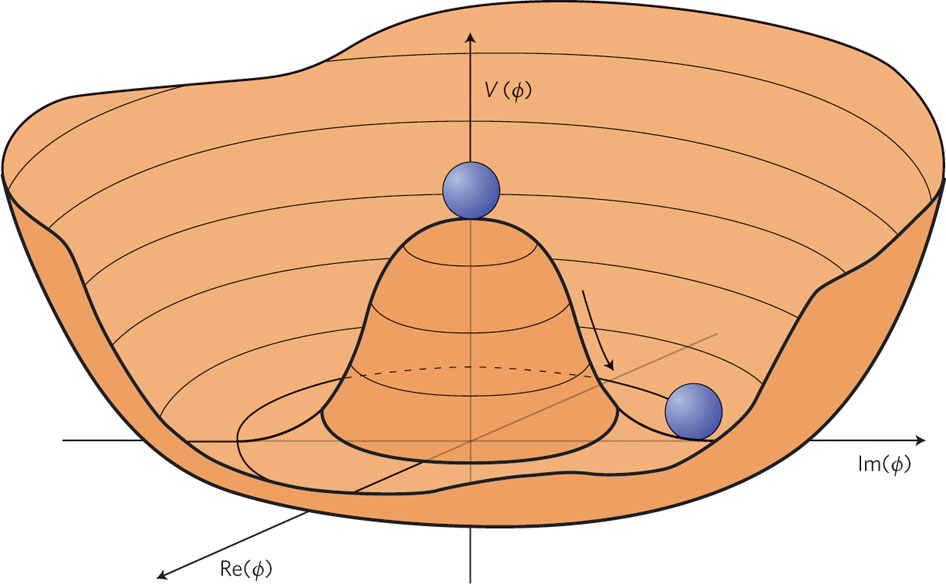
\includegraphics[width=0.6\textwidth]{Figures/Theory/MHat}
\caption[The Higgs potential chosen where $\mu^{2} < 0, \lambda > 0$ introducing degeneracy and breaking the electroweak symmetry into that of QED.]{\label{fig:MexicanHat}The Higgs potential chosen where $\mu^{2} < 0, \lambda > 0$ such that the minimum does not exist at 0, but instead in a ring of infinite minima about zero, thus introducing degeneracy and breaking the electroweak symmetry into that of QED.~\cite{MexHat}}
\end{figure}

The distinction between the two forces caused by this symmetry breaking are due to a linear combination of the weak hypercharge, Y, and isospin component, $T_{3}$, that vanishes for the Higgs. As this defines the conserved quantity $Q$ for the electromagnetic group, this is not affected by the Higgs, and thus the $U(1)_{em}$ group remains unbroken. Conversely, the weak portion interacts with the Higgs and the W$\pm$ and Z bosons acquire mass.  

\section{Motivation for Physics Beyond the Standard Model}
The standard model has been widely successful, predicting the existence of particles such as the $W^{\pm}$ and Z Bosons, and the t quark, showing impressive agreement with experimental findings at the level of 0.1\%. However, there are several signs that it is not a complete theory, and that more information is needed to describe physics at higher energy scales. On the theoretical side, it is dissatisfying that the SM does not currently incorporate the gravitational force, or explain the existence of dark matter or dark energy. Neutrino masses and flavour mixing are also unexplained, and the Higgs is, as yet, undiscovered. In addition it requires several input parameters to tune the masses of particles and flavour mixing, generally viewed as inelegant, as this relies on experimental data and thus does not provide a simple, fundamental picture of nature.  The existing SM is therefore generally thought of as an effective theory, a very low energy approximation to a more complete theory\cite{PeskinSch}.

The incorporation of the gravitational force has not bothered particle physicists much at the electro-weak energy scale as the strength of the effects of gravity on fundamental particles is negligible compared to the other fundamental forces. However, at an energy known as the Planck Scale, $M_{p} \sim 10^{18}$\,GeV, quantum gravitational effects become important, leading to the breakdown of the existing QFT picture of the Standard Model. Thus new physics must exist at this energy scale, or before, indicating the SM is only valid up to some unknown energy scale. In the event that no new physics exists prior to the Planck scale, the Higgs mechanism theory requires fine-tuning to lower the Higgs mass, which is considered to be ``unnatural". This is known as the ``hierarchy problem", discussed in depth below.

As there are both theoretical and experimental concerns over the SM the construction of Beyond the Standard Model (BSM) theories are provoked, many of which come in to play at the TeV scale which is accessible for exploration for the first time with the LHC. A detailed description of a few of the most interesting shortcomings relevant to this thesis are given below.

\subsection{The Hierarchy Problem}
Although the Higgs Boson has yet to be observed experimentally, its mechanism is necessary to the Standard Model to provide mass to the particles, and thus is considered to exist unless proven otherwise. However, while it solves the spontaneous symmetry breaking problem, the Higgs theory introduces theoretical issues of its own. The presence of the Higgs in the SM ensures the WW scattering amplitude does not violate unitarity, but only whilst the $m_{H} < 1$~$\textrm{TeV}$, providing an upper bound on the expected mass~\cite{WWHMass}. 

However, the mass of the Higgs given by its self interaction receives extremely large radiative corrections. This is due to the heavy fermion--anti-fermion pair loop contribution, seen in Figure \ref{fig:hiloop}. 

\begin{figure}
\centering
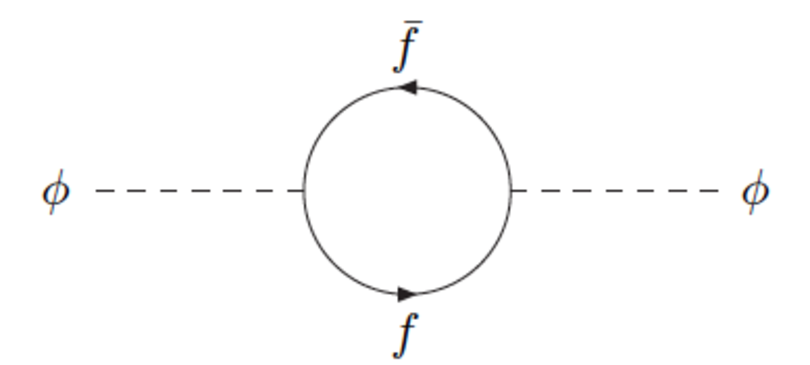
\includegraphics[width=0.4\textwidth]{Figures/Theory/higgsself}
\caption{\label{fig:hiloop}The loop contribution to the Higgs self-mass interaction from fermion-anti-fermion pairs in the SM}
\end{figure}

If each coupling with a fermion, $f$, has a term in the Lagrangian $-\lambda_{F} H \bar{f}f$, it contributes a quadratically divergent factor $\delta m^{2}_{H}$ that corrects the squared mass of the Higgs. 

\begin{equation}
\delta m^{2}_{H} =\sum_{f} - \frac{|\lambda_{f}|^{2}}{8 \pi^{2}}\Lambda^{2}_{UV} + \mathcal{O}(ln\Lambda)
\label{eqn:HIGGQUAD}
\end{equation}

The factor $\lambda_{f}$  represents the coupling for each type of fermion, which is largest in the case of the top quark, where $\lambda_{t} \approx. 1$. The parameter $\Lambda_{UV}$ is the \textit{ultraviolet cutoff}, so named as it represents the smallest distance probed in the calculation. It can be thought of as the scale up to which the Standard Model is valid, as any new physics would change the theory.

 If there were no new physics at a lower energy, the parameter $\Lambda$ takes the value of the Planck Scale $M_{P}$, but in this case the correction will be 30 orders of magnitude higher than the 1 TeV upper bound justified experimentally~\cite{Drees}. As there exists nothing in the SM to fix the Higgs mass, the theory requires fine-tuning, tweaking the parameters to agree with observational findings. This is generally accepted to be an inelegant method, as it requires the input of extra information, and indicates a gap in the fundamental description leading to searches for extensions to the Standard Model. 

\subsection{Cold Dark Matter}

The existence of Dark Matter was postulated as early as 1933 by Fritz Zwicky~\cite{zwicky}, as the orbital velocities of galaxies in clusters were inconsistent with their observed mass, suggesting some additional mass was present but not luminous.  Measurements of rotation curves of galaxies, cosmic microwave background and structure formation have confirmed this concept over the years. Experimental results from WMAP conclude only $\sim 4.5\%$ of the energy in our universe is made of the baryonic matter we see, while dark matter accounts for $\sim 23\%$ and the rest is comprised of another unknown, dark energy~\cite{WMAP5}. Although the existence of such matter has been well documented, there is still no understanding of the physics behind the phenomena. In order to explain the properties a weakly interacting massive particle (WIMP) is required, and it must be electrically neutral. There is no provisions for such a particle in the SM, indicating additional particle content requiring extensions in the theory. 

\subsection{Unification of Coupling Constants}

At the basis of theoretical particle physics is the observation of the symmetry and simplicity of nature. Unification, where several theories can be combined into one description, is desirable and has occurred previously in scientific history, first between electricity and magnetism, and then electromagnetism with the weak force. While each of the three forces of the SM have their own coupling constant, as the energy scale is increased the coupling constants converge towards one another. However precision measurements show that within the current framework,  there is no common point where all three intersect simultaneously. In addition, at the Planck Scale as gravity's coupling constant would be of similar strength many hope for a Grand Unified Theory (GUT),  occurring at this scale known also as the GUT scale. This is only possible with the incorporation of some new physics which would alter the trend of the couplings between the electroweak scale and this GUT scale. 



\section{Supersymmetry}

These major issues with the SM theory suggest a higher energy extension to the current theory is required. There are several possible options, but this thesis will focus on the theory that many consider offers the best solution to the three issues highlighted and discussed in detail, beginning with a natural way to eradicate the hierarchy problem simply and without fine tuning.

The hierarchy problem could be removed, rather than controlled, if there were a way to cancel out the quadratic diverging term in the Higgs mass correction. As the correction for bosons has the opposite sign, the concept of a new symmetry was born, one between fermions and bosons. Known as SUperSYmmetry (SUSY), this theory extends the SM under this symmetry such that elementary particles in the SM each have a superpartner, known as a sparticle, differing by one half unit of spin and is as yet undiscovered, just as the anti-particles were once postulated. Each SM fermion has a boson partner and every SM boson a fermion partner. 

For every fermion contributing to the quadratic divergence, a boson partner contributes an equal and opposite term, and thus the hierarchy problem could cancel out and the mass of the Higgs can take a sensible value. At the heart of supersymmetry is a transformation that changes the field of a fermion into that of a boson, and vice versa. The generator of the transformation shall be known as Q,

\begin{equation}
\textrm{Q}|\textrm{fermion}\rangle = |\textrm{boson}\rangle,  \; \; \; \;  \textrm{Q}|\textrm{boson}\rangle = |\textrm{fermion}\rangle  
\label{eqn:Q}
\end{equation}

where the complex spinors that generate SUSY anti-commutate, with the following relationships where $P^{\mu}$ is the generator of space-time translations and indices are suppressed:


\begin{equation}
\{\textrm{Q},\textrm{Q}\} = \{\textrm{Q}^{\dagger},\textrm{Q}^{\dagger}\} = 0 \qquad \{\textrm{Q},\textrm{Q}^{\dagger}\} = P^{\mu} 
\end{equation} 


In addition to its neat solution to the hierarchy problem SUSY has several other consequences which lead to its position as a favoured theory for new physics at the TeV scale. The addition of SUSY particles to the SM has the side effect of altering the runnings of the gauge coupling constants of the three fundamental forces. Figure \ref{fig:couple} shows the running constants from the SM alongside those with the SUSY model incorporated. Whilst the SM allowed only two to intersect at any point, SUSY alters them such that they are consistent with theories of Grand Unification, as the three are equal at the GUT scale $Q$ $\sim 10^{16}$ GeV. 

Rather than a motivation, this is a pleasant coincidence, but lends plausibility to the theory. It also shows promising features necessary for theories to incorporate gravity, although it does not finish the job. SUSY itself cannot be the final fundamental theory of particle physics, but is an extension which shows much promise, and is a pre-requisite for many higher energy theories such as most formulations of String Theory~\cite{Dine}. The final, perhaps most exciting feature of SUSY is that it can offer a candidate for the particle that represents dark matter with the introduction of a new quantum number $R$ - Parity. 

\begin{figure}
\centering
\subfigure{\label{snk}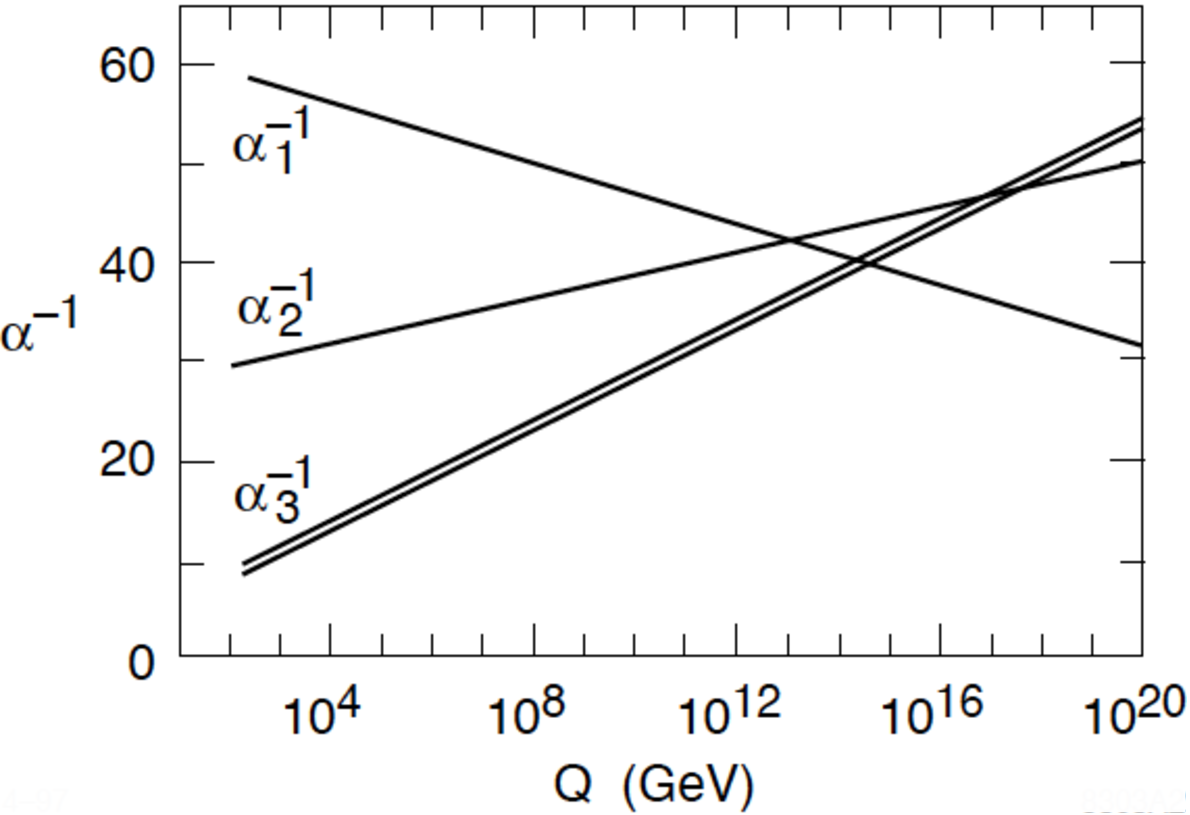
\includegraphics[width=0.40\textwidth]{Figures/Theory/smcoupling}}
\subfigure{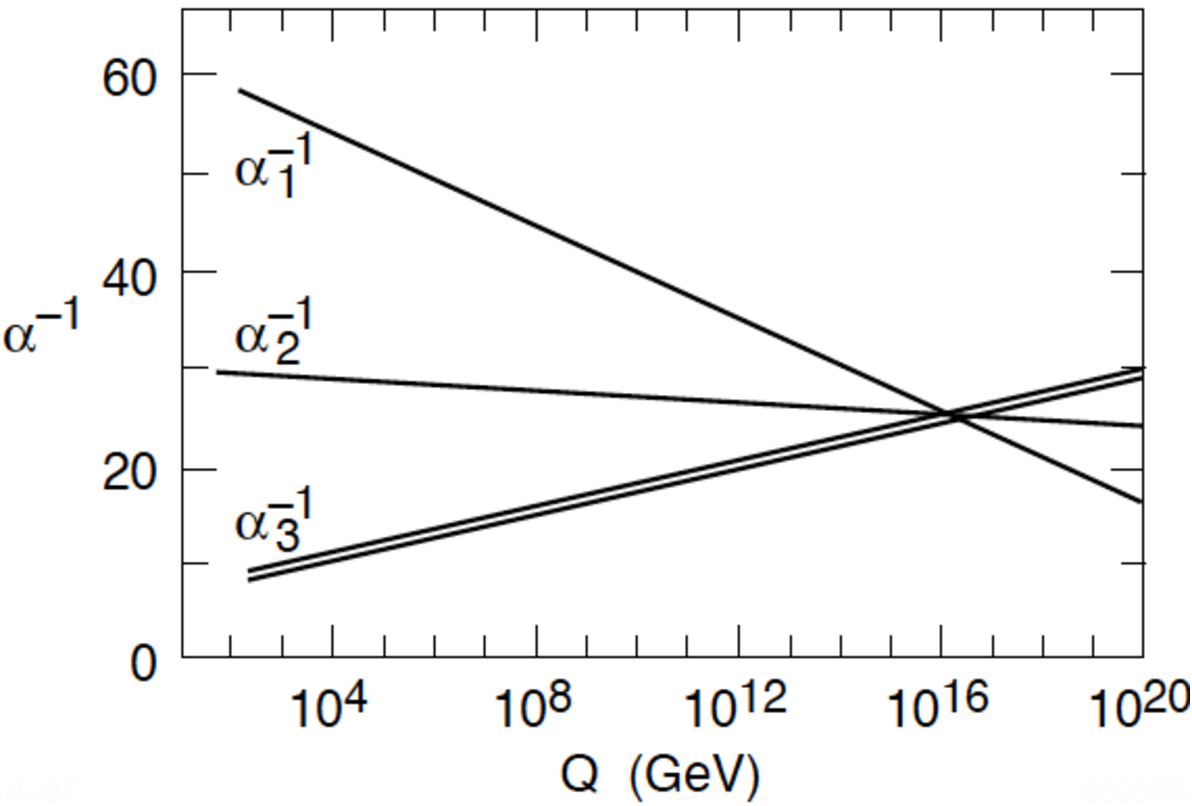
\includegraphics[width=0.40\textwidth]{Figures/Theory/susycoupling}}
\caption[The running gauge coupling constants for $SU(3)_{C} \times SU(2)_{L} \times U(1)_{Y}$ in the SM and SUSY cases.]{\label{fig:couple}(a) The SM running gauge coupling constants for $SU(3)_{C} \times SU(2)_{L} \times U(1)_{Y}$ are shown with increasing energy scale Q. (b)same plot is made after the supersymmetric extension to the Standard Model has been applied. The double lines for $\alpha_{3}$ indicate the error in experimental  measurement, which is negligible for the other two.~\cite{PeskinBSM}}
\end{figure}



\subsection{$R$-Parity}

Constructing the most general form of SUSY, terms appear which allow processes which violate the conservation of two quantum numbers, the baryon number, $B$, and the lepton number, $L$. Whilst there is no theoretical reason for this to be a problem, these interactions have not been observed, and are constrained heavily. An undeniable constraint is the lifetime of the proton where no decay has been observed indicating it is very large, whereas these processes would facilitate its decay. While $B$ and $L$ are not fundamental symmetries in this theory, it is possible to construct a new quantum number, $R$, defined in Equation \ref{eqn:RPAR} which can be required as a symmetry $R$-parity\cite{terning}. It distinguishes between particles from the SM and the sparticles introduced by SUSY, as under this construction, all SM particles carry $R$ of +1 and all super partners carry -1. 

\begin{equation}
R = (-1)^{3(B-L)+2S}
\label{eqn:RPAR}
\end{equation}
Whilst terms in the Quantum Field Theory do allow for the possibility of violation of this parity, experimental measurements have excluded this for sparticles with masses on the TeV scale, and therefore those within the reach of the LHC. Thus the  majority of searches consider models with a symmetry which forbids this violation and conserves $R$. Several phenomenological consequences that transcend specific models arise from this assumption which provide the backbone to SUSY searches at the LHC:

\begin{itemize}
\item{In order for SUSY particles to be produced at the LHC under this assumption, they must be pair produced from SM particles.} 

\item{The heavier particles will cascade down a decay chain ending through creation of the lightest of the supersymmetric particles, denoted the Lightest Super Partner (LSP)}

\item{The LSP must be stable as it cannot decay into SM particles, and through cosmological bounds must be electrically neutral.} 
\end{itemize}
These characteristics of the LSP show us that it is a WIMP, the type of particle that is sought in Dark Matter searches.  Particles of this type will not interact in a detector, therefore are characterised in an experiment as large amounts of missing energy. As this is directly a characteristic of a WIMP in the final state, such a signature represents not only SUSY but is shared by other new physics models with a dark matter candidate particle. 

Models may be constructed to constrain the violation of B and L without R-parity conservation, but those shall not be considered in this thesis, as this unique feature provides both physical motivation and a search strategy for physics at the LHC.


\subsection{MSSM} 

There are many ways to construct mathematically the theory of Supersymmetry, but it is usual to do so in a way which introduces the least number of new degrees of freedom. This demands the minimal particle content required to satisfy the core symmetry, which corresponds to one new degree of freedom for each existing SM one. This approach is known as the Minimal Supersymmetric Standard Model (MSSM), and has an additional new particle, known as a sparticle, for each known SM particle. 

The particles are arranged to fit the irreducible representation of the symmetry, in \textit{supermultiplets}, each of which contains both fermions and bosons. The number of bosonic and fermionic degrees of freedom are therefore equal in any supermultiplet. There are two types of supermultiplet available, a chiral supermultiplet which describes a left-handed fermion, its right handed anti-particle, a complex boson and its conjugate, and a vector multiplet - a massless vector field and a left handed fermion, which result in the fermion and its anti-particle and two transversely polarised vectors bosons\cite{SUSYPrime}. 

The names of the spin-0 bosons that partner the SM fermions are prefixed with ``s-", known as squarks and sleptons, collectively the sfermions. As the SM contains a distinction between left and right handed fermions, the boson super partners have one of each too, and are labelled RH and LH, but it is important to remember this is not a description of the super partner itself, merely a label to describe the SM particle it is associated with. The particles are written with a tilde above the SM symbol so the top quark, t, becomes the ``stop" quark, $\tilde{\textrm{t}}$.

The names of the fermions from the SM bosons are appended with ``-ino" such as the super partners of the gluons, the gluinos. However, for the other fundamental SM bosons, identifying their super-partners is not so simple. The symmetry acts not on the results of electroweak symmetry breaking but on the fields of the $SU(2)_{L} \times U(1)_{Y}$ group. Thus there should be three Winos \~{W} and a Bino \~{B}. 

The Higgs receives different treatment in SUSY than that discussed earlier for the SM, where the scalar field gives up three degrees of freedom to give mass to the vector bosons W$^{\pm}$ and Z. In SUSY, instead two supermultiplets with differing quantum number are required to maintain the electroweak symmetry breaking, one chiral and one vector. These give mass respectively to the up-type quarks of charge $+\sfrac{2}{3}$ and the down-type quarks of charge$-\sfrac{1}{3}$, and thus are named $H_{u}$ and $H_{d}$~\cite{SUSYsuch}. Where the SM has one complex doublet, the MSSM has two complex Higgs doublets, hence the sector has 8 degrees of freedom. Three are lost to give the W$^{\pm}$ and Z bosons mass in electroweak symmetry breaking, leaving five which represent five Higgs boson particles: the charged Higgs bosons $H^{\pm}$, and three neutral bosons h, H and A. The corresponding super-parters are known as the Higgsinos.  


\subsection{Supersymmetry Breaking}

In order to satisfy an exact symmetry, one would expect that each super-partner would have the same characteristics as its SM partner, including its mass. This would indicate they were within the reach of previous physics experiments, but manifestly this is not true as there has been no experimental evidence of particles in the energy spectra previously covered by experimental research. Drawing parallels with the problem of electro-weak symmetry breaking, it is said SUSY is broken by some mechanism, resulting in particles with heavier masses than their counterparts. Although the size of these masses could theoretically take any value, in order for SUSY to eliminate the hierarchy problem this breaking must occur at the Electroweak Scale, which puts an upper bound on the mass differences of around 1 TeV.  

This is known as ``soft" SUSY breaking, and offers the hope of discovering such new physics at the TeV scale, as is now possible for the first time with the LHC. This involves ``soft" mass terms being incorporated into the Lagrangian theory that do not introduce quadratic divergences leading to a new "hierarchy problem". However, the nature of this breaking is not known and thus it is traditional to formulate it in the theory to contain all the mass and mixing terms allowed by the underlying symmetry, which gives arbitrary masses to the sparticles. As there are many unknowns this introduces a large number of parameters to the system. Not all is lost, as SUSY is still capable of making useful predictions, however to complete the theory an understanding of the nature of SUSY breaking is really required. 

Due to electroweak symmetry and soft SUSY breaking the fermions super-partners of the $SU(2)_{L} \times U(1)_{Y}$ group are not generally the mass eigenstates. Instead the winos and bino mix with the Higgsino fields to produce the mass eigenstates in two groups, the charginos $\tilde{\chi}^{\pm}_{1,2}$ and the neutralinos $\tilde{\chi}^{0}_{1,2,3,4}$


\subsection{Minimal Supergravity and the Constrained MSSM}

Even assuming a minimal particle content, the MSSM has a large number of free parameters, introduced through SUSY and Electroweak symmetry breaking, 105 new parameters in addition to the 19 already present in the SM. When it comes to experimental searches, this is an unworkable number, for to examine possible behaviour of SUSY one would have to look in 105 dimensions. Thus for the purpose of constructing models to work with, it is desired to constrain the number of free parameters in the theory. One well-motivated method of constraint is the GUT model theory of minimal SUper GRAvity, otherwise known as mSUGRA. 

The many parameters of the MSSM are in fact not all constants, but rather vary with the energy scale. Thus, to constrain the model the assumption can be made that there is some ``hidden sector" (perhaps of the order of the $M_{P}$) which contains fields with no couplings to what is now thought of as the ``visible sector" of the MSSM. There should then be some messenger between the two, that allows supersymmetry breaking to be mediated by the MSSM in order to provide the soft terms. In the mSUGRA theory the nature of this messenger is that it is ``gravity mediated". 

The MSSM combined with the theory of mSUGRA is called the Constrained MSSM, or CMSSM, as the number of free parameters is reduced to a manageable five. These factors are:

\begin{itemize}
\item{A common scalar mass, $m_{0}$}
\item{A common gaugino mass, $m_{1/2}$}
\item{The SUSY Breaking common trilinear coupling, $A_{0}$}
\item{The ratio of the vacuum expectation values of the two Higgs fields, tan $\beta$}
\item{ The sign of the Higgs parameter, sign($\mu$)}
\end{itemize} 

With this relatively small parameter space it is possible to construct models with which to design search strategies, and allows us the exclusion of regions with the advent of new results. A given point in mSUGRA space defines the mass hierarchy of the squarks, gluinos, charginos and neutralinos, therefore governing the interactions that are possible, as well as the identity of the LSP. Thus, in different regions the productions mechanisms can differ, however in the majority of phase space the LSP is the lightest of the neutralinos, $\tilde{\chi}^{0}_{1}$.  For convenience, mSUGRA is shown graphically in the $m_{0}$ - $m_{1/2}$ plane, for set values of the other three parameters. 

There are other theories that support mechanisms of SUSY breaking, such as Gauge-Mediated Symmetry Breaking (GMSB) and Anomaly Mediated Symmetry Breaking (AMSB) but these are not considered for the purpose of this thesis. 

\subsubsection{Current Limits on the CMSSM}

Two types of limits exist in mSUGRA space, those imposed theoretically and those that result from experimental data. Of the latter, some are contributed by cosmology, and others by particle physics. 

There are some regions of the parameter space where the masses of the particles have a hierarchy which results in the stau being the LSP. This is theoretically forbidden as the LSP certainly contributes some if not all of the dark matter in the universe, and it is known to be neutral. 

In addition, a further region is excluded whereby the the LSP would be inconsistent with the WMAP measurement of the Dark Matter relic density. 

\subsection{Production Mechanisms in p-p collisions}
With a proton-proton collider at TeV energies such as the LHC, as discussed before we can consider the protons as a set of partons each carrying a fraction of the total momentum. It is these quarks and gluons that collide. At such high energies these can be from the gluons in the sea as well as the valence quarks, thus there are qq, $\textrm{q}\bar{\textrm{q}}$, qg and gg collisions to consider.
Assuming SUSY exists within the reach of the LHC, indicated by the restriction imposed on the mass differences of SUSY breaking, then from these interacting pairs large production rates of both squarks and gluinos are expected. Cross sections in the region of 100 pb to 1fb are possible for SUSY sparticles with masses between 0.5 TeV and 1 TeV~\cite{early}. Predominantly the production is the result of strong processes resulting in squarks and gluinos, although weak production is predicted albeit at smaller cross sections. Decays from these particles through charginos and neutralinos would result in production of the LSP, but the structure of these decays depends on the mass hierarchy of the sparticles, which is determined by the values of m$_{0}$ and m$_{1/2}$.  Thus a chosen point in this plane represents a certain set of kinematics. SUSY production in these collisions is dominated by the pair-productions $ qq \rightarrow \tilde{g} \tilde{g}, \tilde{q}\tilde{g}, \tilde{q} \tilde{q}$. The relative cross sections of these decay modes depend on the region of mSUGRA 

\begin{figure}
\centering
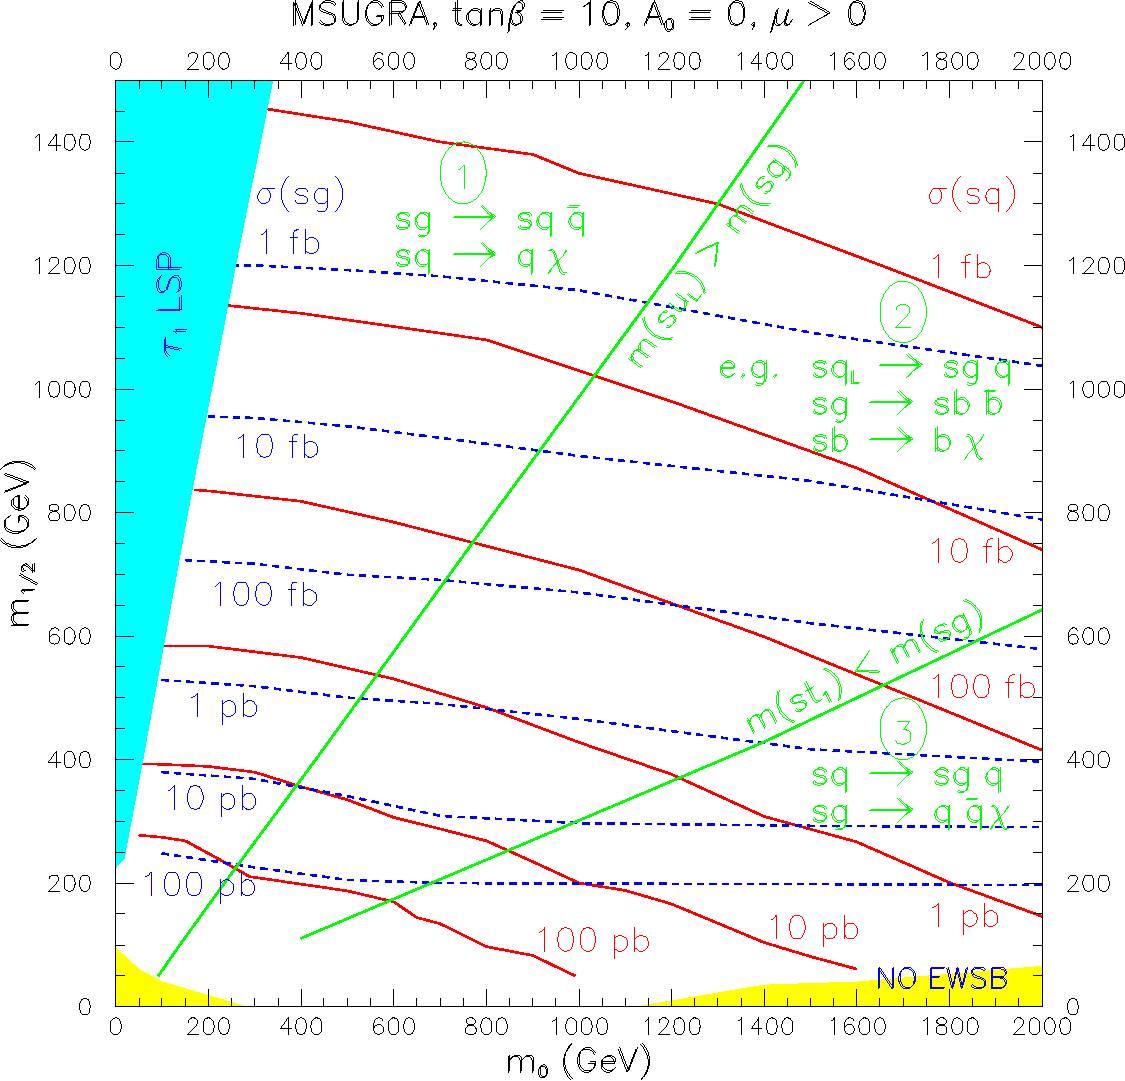
\includegraphics[width=0.6\textwidth]{Figures/Theory/mSUGRA_TDR_1}
\caption[The $m_{0}-m_{1/2}$ plane of mSUGRA depicting diagonal lines separating three distinct regions of mass hierarchies based on the mass difference of squarks and gluinos. ]{\label{fig:msugratdr}The $m_{0}-m_{1/2}$ plane of mSUGRA depicting diagonal lines separating three distinct regions of mass hierarchies based on the mass difference of squarks and gluinos. Lines of constant production cross section for squarks and gluinos are shown in red and blue respectively. The allowed decays in each region are shown, where ``sq" denotes a squark, and ``sg" a gluino.\cite{CMSTDRII}}

\end{figure}

Within mSUGRA there are three distinct regions which exhibit different decay modes, defined by the mass relationship between the gluinos and the squarks. These can be seen in Figure \ref{fig:msugratdr}, where the diagonal green lines represent a cross-over in the squark-gluino hierarchy. Passing left-right on the diagram, the regions are:

\begin{description}
\item[Region1: $m_{\tilde{g}} > m_{\tilde{q}}$]{As the gluinos are heavier than the squarks, the general form of decays producing $\chi$, the set of charginos and neutralinos, is
\begin{equation}
\tilde{g} \rightarrow \tilde{q} \bar{q} , \tilde{q} \rightarrow q \chi
\end{equation}
}
\item[Region 2: $m_{\tilde{g}}< m_{\tilde{q}_{L}}, m_{\tilde{g}}> m_{\tilde{t}_{1}} $]{Here the mass of the gluino lies between that of the heaviest and lightest squark, therefore more complicated decay relationships between the two are allowed, and these depend on exactly which squarks are heavier and which lighter. The $\tilde{q}_{L}$ are the heaviest, while states such as $\tilde{b}_{1}$ and $\tilde{t}_{1}$ are some of the lightest. The heavier squarks decay to lighter squarks and to gluinos, and the gluino decays to lighter squarks. }
\item[Region 3: $m_{\tilde{g}} < m_{\tilde{q}}$]{Finally in this region the gluino is lighter than any squark, and the allowed decays take the form
\begin{equation}
\tilde{q} \rightarrow \tilde{g}q , \tilde{g} \rightarrow q\bar{q} \chi
\end{equation}
}
\end{description}

As the dominating decay of both squarks and gluinos produce quarks, it is expected in a SUSY event many hadronic jets from these sources along with the gluon radiation from the incoming and outgoing partons. Thus a traditional R-parity conserving SUSY signature that provides the basis for this thesis is that of multiple jets and evidence of a (missing) LSP. 



